\chapter{\textit{Software} 'Pé na Estrada'}
  
  Esse capítulo traz informações sobre o \textit{software} Pé na estrada, apresentando o modelo de dados fornecido pela PRF
  pela lei dos dados abertos, uma breve explicação das funcionalidades e estruturação atual do \textit{software} e finalizando 
  com as possíveis mudanças no \textit{software} com a utilização da ontologia.
  
  \section{Dados abertos}
  
    
Os dados são disponibilizados, semestralmente, em planilhas baseadas no modelo da
Figura \ref{fig:modelo_prf}, e para obter dados específicos de cada acidente, as informações precisam ser
correlacionadas entre tabelas, que podem ser vistas na Figura \ref{fig:tabela_dados}. As planilhas também contêm
uma grande quantidade de dados, pois são divulgados cerca de 45.000 acidentes por semestre,
além de uma quantidade exagerada de tabelas para o relacionamento, pouco eficiente, dos
dados.

\begin{figure}[!htb]
 \centering
 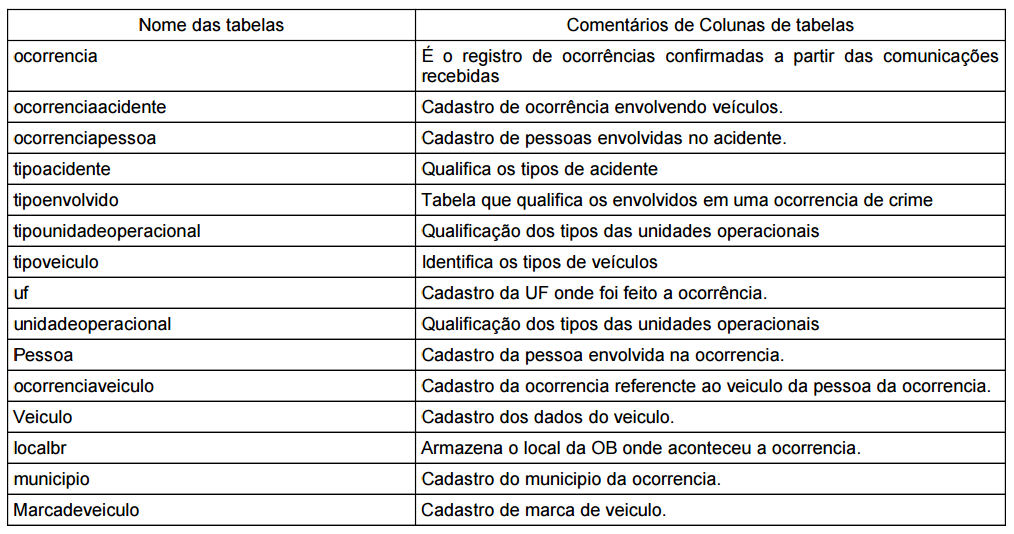
\includegraphics[scale = 0.4]{tabela_dados}
 \caption[Tabelas da base de dados da PRF]{Tabelas da base de dados da PRF. Fonte: \cite{brasil13}}
 \label{fig:tabela_dados}
\end{figure}

\begin{figure}[!htb]
 \centering
 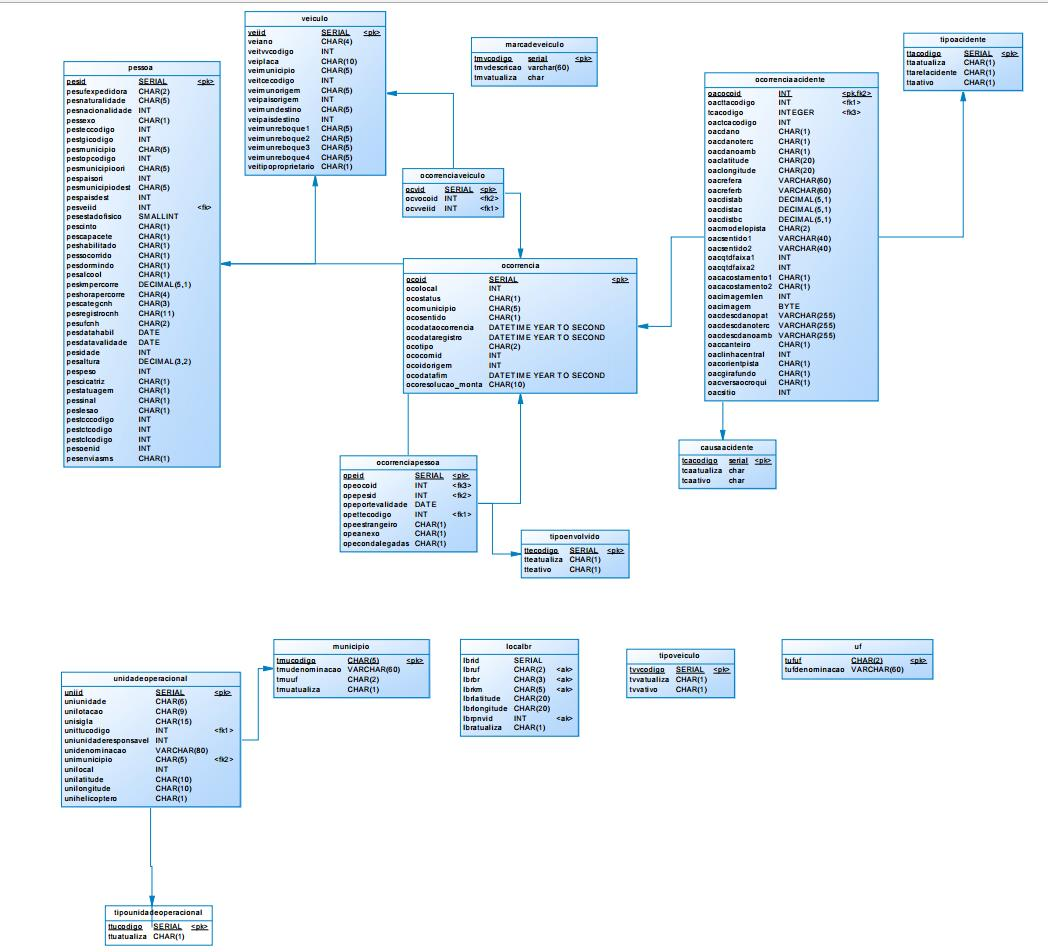
\includegraphics[scale = 0.4]{modelo_prf}
 \caption[Modelo de Dados atual das Ocorrências de Acidentes em Rodovias Federais]
  {Modelo de Dados atual das Ocorrências de Acidentes em Rodovias Federais. Fonte: \cite{brasil13}}
 \label{fig:modelo_prf}
\end{figure}
  
  \section{Pé na estrada}
    A disponibilização das ocorrências de acidentes em rodovias federais através da PRF,
    embora exista, não é realizada de forma visual. Todavia, consiste na disponibilização de
    planilhas complexas que contém muitos dados.

    O software “Pé na estrada” foi desenvolvido, utilizando os dados divulgados pela
    PRF, com a finalidade de apresentar essas informações de forma mais atrativa e visual. Dessa
    forma, é um sistema que permite buscar informações sobre as rodovias federais, visualizando
    as rodovias com maiores índices de acidentes. A aplicação também permite traçar rotas para
    visualizar os trechos mais perigosos, e os acidentes ocorridos ao longo da rota. Há também a
    possibilidade dos usuários fazerem comentários sobre as rodovias. Algumas imagens do
    software podem ser vistas no Anexo A.

    Os dados disponibilizados possuem muitas informações acerca do acidente, como tipo
    do acidente, dano causado à rodovia e tipo de veículo. Contudo, esse tipo de informação não
    foi tratado na aplicação, pois esses dados estavam estruturados de forma complexa e
    inconsistente. Os relacionamentos entre os dados eram feitos por meio de uma grande
    quantidade de tabelas relacionadas, o que dificultaria a apresentação desses dados na
    aplicação, tornando o sistema lento e demasiado complexo de se manter. O modelo de dados
    utilizado na aplicação pode ser visto na Figura \ref{fig:modelo_penaestrada}.

    \begin{figure}[!htb]
    \centering
    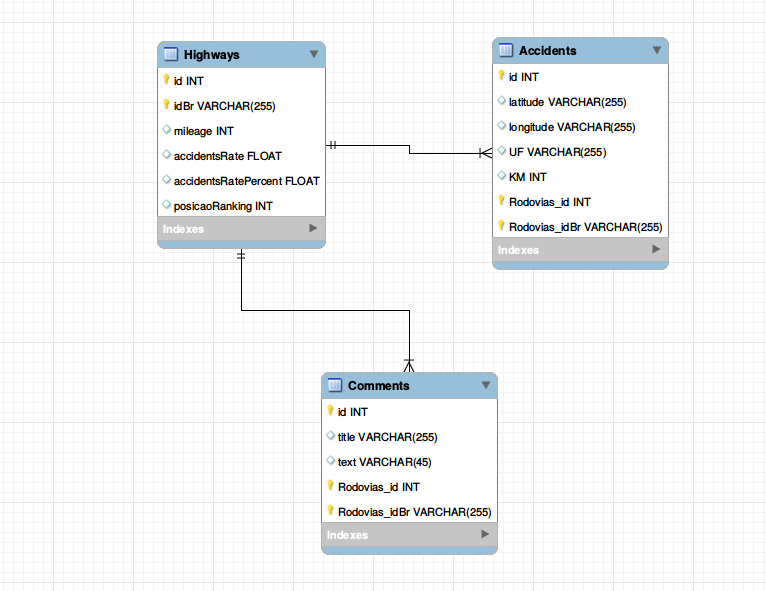
\includegraphics[scale = 0.4]{modelo_penaestrada}
    \caption[Modelo de dados do \textit{software} “Pé na Estrada”]{Modelo de dados do software “Pé na Estrada”.}
    \label{fig:modelo_penaestrada}
    \end{figure}

      \subsection{Planejamento da aplicação da ontologia no ``Pé na Estrada''}

Atualmente, o “Pé na estrada” disponibiliza informações apenas sobre os locais dos
acidentes, e a quantidade de acidentes em cada rodovia. Esse tipo de informação seria mais
relevante se acompanhassem informações acerca dos tipos de acidentes, danos causados a
rodovia, tipo de veículo, envolvidos, entre outros dados que fossem relevantes para análise
estatística e para representação gráfica.

Dessa forma, com o modelo de dados estruturado semanticamente, esses dados seriam
encontrados e relacionados facilmente, possibilitando ao software disponibilizar essas
informações ao usuário, até mesmo de forma mais visual.

Atualmente, o software não possui nenhuma camada semântica presente, possuindo
apenas a camada visual do HTML, sendo necessária toda a estruturação das três principais
camadas semânticas: o XML, o RDFS e a OWL, sendo esta última necessária para o uso da
ontologia que será criada para representar os acidentes de trânsito.

O software ``Pé na Estrada'' foi desenvolvido na linguagem \textit{Ruby} com a utilização do \textit{framework Rails}. 
A partir disso, o sistema funciona com a arquitetura da Figura \ref{fig:arquitetura}

\begin{figure}[!htb]
 \centering
 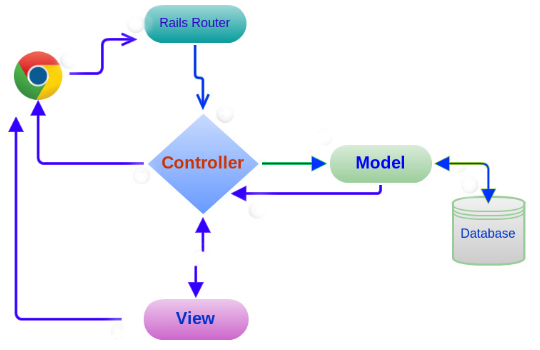
\includegraphics[scale = 0.7]{figuras/arquiteturarails.png}
 \caption{Arquitetura do sistema}
 \label{fig:arquitetura}

\end{figure}

O \textit{Rails router} é responsável por estabelecer routas que comunica o sistema com o navegador. Essa rota é obtida
na \textit{Controller} que a partir disso gera a \textit{View}. Os dados são obtidos e armazenados na base de dados através da \textit{Model}
que extende do \textit{Active Record} que é a classe responsável por fornecer os meios de comunicação com a camada de dados.

Para fazer a comunicação da aplicação com a ontologia definida é necessário substituir a comunicação da \textit{Model} que ao invés
de estabelecer relação com a \textit{Active Record} deve estabelecer relação com dados em RDF.

Existe um \textit{framework} chamado \textit{Active RDF} \footnotemark[1] que substitui a \textit{Active Record} e estabelece um relacionamento
do sistema com os dados contidos na ontologia. 

\footnotetext[1]{http://www.activerdf.org/}
  
